\documentclass[12pt]{article}

\usepackage{anyfontsize}
\usepackage{enumitem}
\usepackage{physics} 
\usepackage{enumerate}
\usepackage{pgfplots}
\usepackage{pgfplotstable}
\usepackage{tikz,pgfplots}
\usepackage{graphicx}
\usepackage{float} 
\usepackage{subfigure}
\usepackage[toc,page]{appendix}
\usepackage{amsmath}  %I added this so that you can use the align tool for equations!
\usepackage{amssymb}
\usepackage{wasysym} %This package allows you to put emojis in your paper!!!!
%wasysym: \smiley{} \frownie{} see http://milde.users.sourceforge.net/LUCR/Math/mathpackages/wasysym-symbols.pdf for list of most symbols available in this package
\usepackage{array}
\usepackage{tabularx}
\usepackage{cellspace}
\usepackage{geometry}
\usepackage{listings}
\usepackage{color}
\usepackage{fontspec}
\usepackage{booktabs}
\usepackage{newtxtext,newtxmath}
\usepackage{caption}

\geometry{
  a4paper,
  total = {170mm, 257mm},
  left = 20mm,
  top = 20mm,
  }

\definecolor{dkgreen}{rgb}{0,0.6,0}
\definecolor{gray}{rgb}{0.5,0.5,0.5}
\definecolor{mauve}{rgb}{0.58,0,0.82}
\lstset{frame = tb,
        language = Python,
        aboveskip = 3mm,
        belowskip = 3mm,
        showstringspaces = False,
        columns = flexible,
        basicstyle = {\small\ttfamily},
        numbers = left,
        numberstyle = \tiny\color{gray},
        keywordstyle = \color{blue},
        commentstyle = \color{dkgreen},
        stringstyle = \color{mauve},
        breaklines = true,
        breakatwhitespace = true,
        tabsize=4}

\renewcommand\lstlistingname{Algorithm}
\captionsetup[lstlisting]{singlelinecheck=false, margin=12pt, labelsep=default, labelfont=default}
%We can also use: labelsep=period or labelsep=spacce, labelfont=default or labelfont=bf

\pgfplotsset{compat = 1.14}
%%%%%%%%%%%%%%%%%%%%%%%%% Again, Don't change anything Above %%%%%%%%%%%%%%%%%%%%%%%%%

\begin{document}

\title{\textbf{{\normalsize Computational Physics Lab}\\
                Homework 1}}
\author{108000204\\
        Yuan-Yen Peng\\
        Dept.\ of Physics, NTHU\\
        Hsinchu, Taiwan}
\date{\today}
\maketitle

\section{Programming Assignments}
  \subsection{$\pi$ calculation}

    In this section, we redo the $\pi$ calculation in the class and run the code with N = 10000, 100000, and 1000000. Then, we use the {\ttfamily\%timeit} command in a jupyter notebook to evaluate the performance. Table\ref{tab1_result} is our result with 3 different methods. The first is to use hand write for-loop; the second is to use the default sum with numpy arrays; the last is to use the numpy sum with numpy arrays. On the other hand, we use $N = 10E3$ to plot the tendency of each methods; also calculate the performance of plotting set value points, i.e., $N = 1, 2 \ldots N$ with Algorithm\ref{per}.

    \begin{lstlisting}[language={Python}, caption={Performance plotting, Three of mehod use the same plotting approach.\label{per}}]
      # cal_meth1 means use method 1
      t1 = time.time()
      X = np.linspace(1, N, N)
      Y = np.array([])
      for i in range (0, N):
        Y = np.append(Y, cal_meth1(int(X[i]))
      t2 = time.time()

      print("time different = ", [t2 - t1])
      print(f"The value is {Y[-1]}"
    \end{lstlisting}

    \renewcommand{\tabularxcolumn}[1]{m{#1}} % set it to the middle of vertical-direction.
    \newcolumntype{A}{>{\raggedleft\arraybackslash}X}
    \newcolumntype{B}{>{\centering\arraybackslash}X}
    \begin{table}[H]
      \centering
      \begin{tabularx}{0.8\textwidth}{BAAA}
      \toprule
      \multicolumn{1}{c}{N} & \multicolumn{1}{c}{method 1}   & \multicolumn{1}{c}{method 2}     & \multicolumn{1}{c}{method 3}    \\[0.1cm]
      \midrule
      $10E4$       & $49.8 ms \pm 805 \mu s $ & $50.8 ms \pm 1.06 \mu s $ & $49.7 ms \pm 721 \mu s $ \\[0.3cm]
      $10E5$       & $493 ms \pm 6.05 ms $    & $502 ms \pm 3.69 ms $     & $485 ms \pm 6.9 ms $    \\[0.3cm]
      $10E6$       & $5.01 s \pm 62.4 ms $    & $5.02 s \pm 99.9 ms $     & $4.9 s \pm 85 ms $    \\[0.3cm]
      \bottomrule
      \end{tabularx}
      \caption{Three different methods for the $\pi$ calculation\label{tab1_result}}
    \end{table}

    \begin{lstlisting}[float, floatplacement=H, language={Python}, caption={Method 1, using default for loop.}]
      for i in range (0, N + 1, 1):
        h = np.sqrt(1 - (i/N)**2)
        area += dx * h

      Area = area * 4
    \end{lstlisting}

    \begin{figure}[H]
      \centering 
      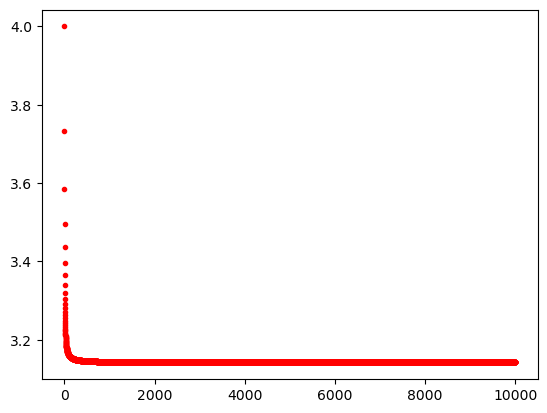
\includegraphics[width = 12cm]{fig1_per.png}
      \caption{Method 1, the performance is approximately 24.22 seconds; the $\pi$ is approaching to the stable value: 3.141791477611317.\label{fig1_per}}
    \end{figure}

    \begin{lstlisting}[language={Python}, caption={Method 2, using default sum.}]
      x = np.linspace(0, 1, N)
      y = np.sqrt(1 - x**2)
      area = sum(dx*y)

      Area = area * 4
    \end{lstlisting}


    \begin{figure}[H]
      \centering 
      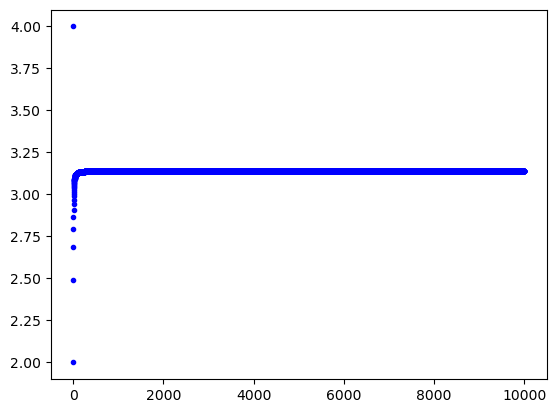
\includegraphics[width = 12cm]{fig3_per.png}
      \caption{Method 2, the performance is approximately 0.31 seconds; the $\pi$ is approaching to the stable value: 3.1414773182871603.\label{fig2_per}}
    \end{figure}

    \begin{lstlisting}[language={Python}, caption={Method 1, using {\ttfamily np.sum}.}]
      x = np.linspace(0, 1, N)
      y = np.sqrt(1 - x**2)
      area = np.sum(dx*y)

      Area = area * 4
    \end{lstlisting}

    \begin{figure}[H]
      \centering 
      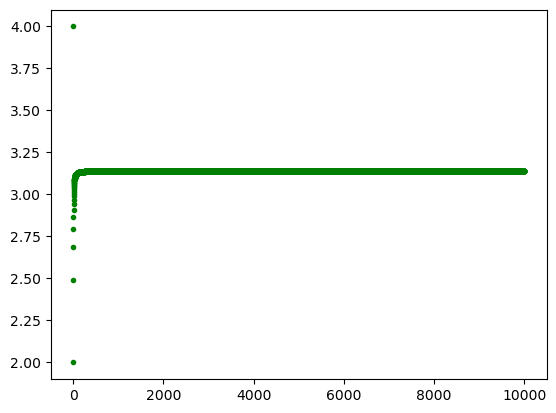
\includegraphics[width = 12cm]{fig2_per.png}
      \caption{Method 3, the performance is approximately 2.40 seconds; the $\pi$ is approaching to the stable value: 3.1414773182871647.\label{fig3_per}}
    \end{figure}

    For results in Table\ref{tab1_result}, with $10E4$, method 2 is the slowest, and method 3 is faster than the others, so we can find that a for-loop for python is slow while it is still faster than the default sum in python; moreover, if using the sum with numpy, the performance of the code will be accelerated. This phenomenon is much more obvious when the N increases, meeting our expectations. In the last class, we have also learned the performance plotting; thus, I use $N = 10E3$ to calculate the performance and also plot it in method 1: figure\ref{fig1_per}, method 2: figure\ref{fig2_per}, method 3: figure\ref{fig3_per}. The performance strongly depends on what methods we use to plot. If we use {\ttfamily numpy.sum} it will be the fastest among the three of them, and if using the for-loop, it will be the slowest, which is not the same as the outcomes of using {\ttfamily \%timeit}. I think that it might depend on how many for-loops we used; that is, when we plot the performance utilizing two for-loops which will degrade the speed much more manifest than taking the default {\ttfamily sum} for only one for-loop. All in all, to summarize the consequences, using a high-speed computing kit, numpy, will significantly speed up our computational performances.
  
  \subsection{Stefan-Boltzmann constant $\sigma_{B}$}
    The method is similar to the $\pi$ calculation. We use the implementation of {\ttfamily numpy.sum} so as to upgrade or speed up computation. In order to avoid the denominator going to zeros leading to the result bursting into infinity, we put in the additional "tolerance"; by doing so, the code can evade this erroneous. According to the hint from the question, we set the upper bound to the $10E15$, as large as we can; lastly get the reasonable result: $\sigma_{B} = 5.6703687488100114E-08$, comparing to the theoretical result: $\sigma_{B} = 5.67037442E-08$.
    
    \begin{lstlisting}[language={Python}, caption={The Stefan-Boltzmann constant $\sigma_{B}$ calculation, performance = $15.6ms \pm 312 \mu s$.}]
        def sigma(N, upper):
        '''
        :param N: divided number.
        :upper: upper bound for infinity, so set it as large as possible.
        '''
        tor_denu = 10E-10
        # lower tolerance math error.
        dNu = upper/N
        Nu = np.linspace(0, upper, N)
        B_nu = 2 * h * Nu**3
        B_denu = c**2 * (np.exp(h * Nu / (k * T)) - 1) + tor_denu
        # lower tolerance (+ 10E-10) to avoid 1/0 (math error).
        sig = np.sum(B_nu * dNu / B_denu) * pi/T**4
      
        return sig
      
      N = int(10E5)
      upper = int(10E15) 
      # as large as we can, because it need to be inf.
      print(sigma(N = N, upper = upper))
      %timeit sigma(N, upper)
    \end{lstlisting}

  \subsection{Angry Brid}
    We set the parameters with playground length $100 [m]$, initial bird's position at $(0.5[m], 0.5[m])$, the pig's position at $(20[m], 1[m])$, and regarding the bird as a circle(2D) and also the pig with radius 0.3 and 0.5 respectively. The method we use is that using another variable, temp, to store the information from the last step. We, afterward, utilize temp to calculate the information of the current step and store them in the specified array. The definition of "success" is within the tolerance of the distance between the target and the bird. We, eventually, get the results in the different mediators showing in the Figure\ref{air1}, \ref{air2}, \ref{water1}, \ref{water2}. Although the outcome is physically correct, the visualizations of the bird(red) and pig(green) are not rendered as the "true" size. Due to the sophisticated settings of {\ttfamily plt.scatter}, I cannot plot the real visualization's results.

    \begin{lstlisting}[language={Python}, caption={This is the algorithm of the simulations of Angry Bird with different circumstances.}]
      def tr(PosX, PosY, Vel, theta, eta):
          VelX = Vel * np.sin(theta)
          VelY = Vel * np.cos(theta)
          K = 6 * np.pi * R
          x, y, vx, vy = PosX, PosY, VelX, VelY # temp
          ax = -K * eta * vx # temp
          ay = -K * eta * vy # temp
          X = np.array([x])
          Y = np.array([y])
          VX = np.array([vx])
          VY = np.array([vy])
          AX = np.array([ax])
          AY = np.array([ay])
          while (x <= D_x and y >= D_y):
                  vy += (-g + ay) * dt # temp
                  VY = np.append(VY, vy)
                  vx += ax * dt # temp
                  VX = np.append(VX, vx)
                  ax = -K * eta * vx # temp
                  AX = np.append(AX, ax)
                  ay = -K * eta * vy # temp
                  AY = np.append(AY, ay)
                  x += vx * dt # temp
                  X = np.append(X, x)
                  y += vy * dt # temp
                  Y = np.append(Y, y)
                  
                  if (np.sqrt(np.square(T[0] - x) + np.square(T[1] - y)) <= PosSec):
                          print('Booom!')
                          break
                  
          return [X, Y, x, y]
    \end{lstlisting}

    \begin{figure}[H]
      \centering 
      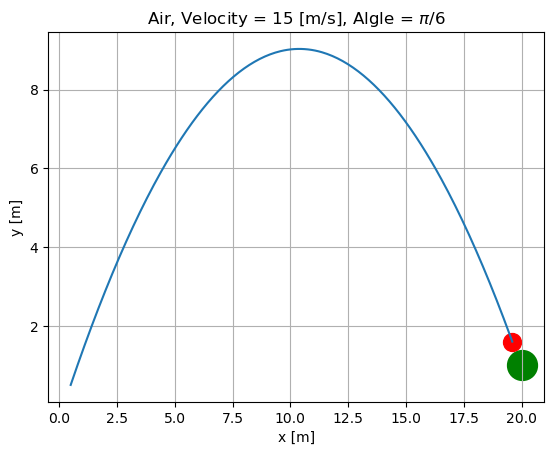
\includegraphics[width = 12cm]{air1.png}
      \caption{If the bird is in the air with $\eta = 2E-4[mks\ unit]$, we can get the successful event with initial speed and angle $(15, \pi / 6) [mks\ unit]$.\label{air1}}
    \end{figure}

    \begin{figure}[H]
      \centering 
      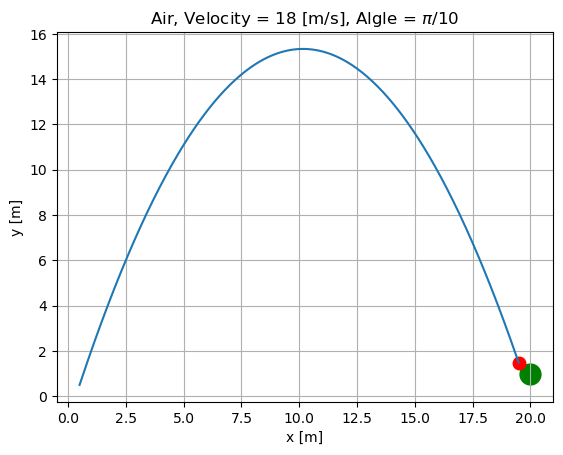
\includegraphics[width = 12cm]{air2.png}
      \caption{If the bird is in the air with $\eta = 2E-4[mks\ unit]$, we can get the successful event with initial speed and angle $(18, \pi / 10) [mks\ unit]$.\label{air2}}
    \end{figure}

    \begin{figure}[H]
      \centering 
      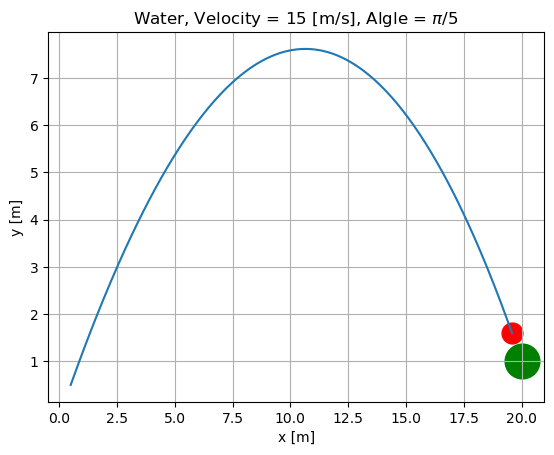
\includegraphics[width = 12cm]{water1.png}
      \caption{If the bird is in the water with $\eta = 0.01[mks\ unit]$, we can get the successful event with initial speed and angle $(15, \pi / 5) [mks\ unit]$.\label{water1}}
    \end{figure}

    \begin{figure}[H]
      \centering 
      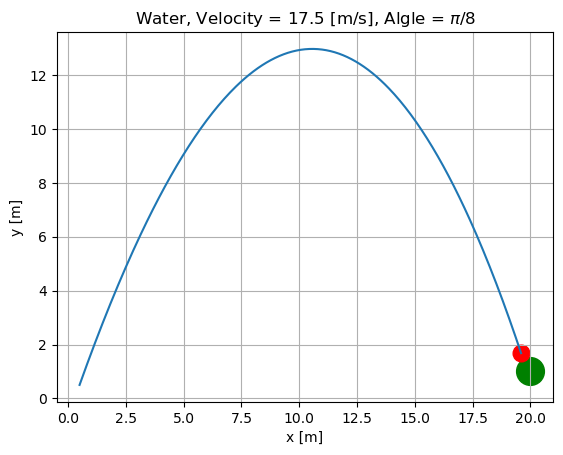
\includegraphics[width = 12cm]{water2.png}
      \caption{If the bird is in the water with $\eta = 0.01[mks\ unit]$, we can get the successful event with initial speed and angle $(17.5, \pi / 8) [mks\ unit]$.\label{water2}}
    \end{figure}

\section{Codes}
    All the codes are transferred from jupyterlab; hence, if you want to re-run them, please see the source code in the attached files or my GitHub repository: <https://github.com/gary20000915/Comphyslab-HW1.git>.
    \subsection{$\pi$ calculation}
      \begin{lstlisting}[language={Python}]
        # %% [markdown]
        # ## Computational Physics Lab 
        # ### Homework 1.1
        # Yuan-Yen Peng   
        # Dept of Physics, NTHU, Taiwan   
        # October 17, 2022   
        
        # %% [markdown]
        # π calculation
        
        # %%
        import numpy as np
        
        N1 = int(10E4)
        N2 = int(10E5)
        N3 = int(10E6)
        # Set how many small rectangles. (divided number)
        
        # %%
        # method 1, use hand writing for-loop.
        def cal_meth1(N: int):
          dx = 1/N
          area = 0
        
          for i in range (0, N + 1, 1):
            h = np.sqrt(1 - (i/N)**2)
            area += dx * h
          Area = area * 4
          
          return Area
        
        print("pi of N = 10000: ", cal_meth1(N1))
        %timeit cal_meth1(N1)
        print("pi of N = 100000: ", cal_meth1(N2))
        %timeit cal_meth1(N2)
        print("pi of N = 1000000: ", cal_meth1(N3))
        %timeit cal_meth1(N3)
        
        # %%
        # method 2, use default sum.
        def cal_meth2(N: int):
          dx = 1/N
          area = 0
          
          x = np.linspace(0, 1, N)
          y = np.sqrt(1 - x**2)
          area = sum(dx*y)
          Area = area * 4
          
          return Area
        
        print("pi of N = 10000: ", cal_meth2(N1))
        %timeit cal_meth1(N1)
        print("pi of N = 100000: ", cal_meth2(N2))
        %timeit cal_meth1(N2)
        print("pi of N = 1000000: ", cal_meth2(N3))
        %timeit cal_meth1(N3)
        
        # %%
        # method 3, use numpy.sum.
        def cal_meth3(N: int):
          dx = 1/N
          area = 0
          
          x = np.linspace(0, 1, N)
          y = np.sqrt(1 - x**2)
          area = np.sum(dx*y)
          Area = area * 4
          
          return Area
        
        print("pi of N = 10000: ", cal_meth3(N1))
        %timeit cal_meth1(N1)
        print("pi of N = 100000: ", cal_meth3(N2))
        %timeit cal_meth1(N2)
        print("pi of N = 1000000: ", cal_meth3(N3))
        %timeit cal_meth1(N3)
      \end{lstlisting}

      The performance code is in the below.
      \begin{lstlisting}[language={Python}]
        # %% [markdown]
        # ## Computational Physics Lab 
        # Yuan-Yen Peng   
        # Dept of Physics, NTHU, Taiwan     
        
        # %%
        import numpy as np
        import matplotlib.pyplot as plt
        import time
        
        N = int(10E3)
        
        # %%
        # method 1, use hand writing for-loop.
        def cal_meth1(N: int):
          dx = 1/N
          area = 0
        
          for i in range (0, N + 1, 1):
            h = np.sqrt(1 - (i/N)**2)
            area += dx * h
          Area = area * 4
          
          return Area
        
        
        t1 = time.time()
        X = np.linspace(1, N, N)
        Y = np.array([])
        for i in range (0, N):
          Y = np.append(Y, cal_meth1(int(X[i])))
        t2 = time.time()
        
        print("time different = ", [t2 - t1])
        print(f"The value is {Y[-1]}")
        plt.plot(X, Y, ".", color = "r", label = "N = 10E3")
        
        # %%
        # method 2, use default sum.
        def cal_meth2(N: int):
          dx = 1/N
          area = 0
          
          x = np.linspace(0, 1, N)
          y = np.sqrt(1 - x**2)
          area = sum(dx*y)
          Area = area * 4
          
          return Area
        
        t1 = time.time()
        X = np.linspace(1, N, N)
        Y = np.array([])
        for i in range (0, N):
          Y = np.append(Y, cal_meth2(int(X[i])))
        t2 = time.time()
        
        print("time different = ", [t2 - t1])
        print(f"The value is {Y[-1]}")
        plt.plot(X, Y, ".", color = "g", label = "N = 10E3")
        
        # %%
        # method 3, use numpy.sum.
        def cal_meth3(N: int):
          dx = 1/N
          area = 0
          
          x = np.linspace(0, 1, N)
          y = np.sqrt(1 - x**2)
          area = np.sum(dx*y)
          Area = area * 4
          
          return Area
        
        t1 = time.time()
        X = np.linspace(1, N, N)
        Y = np.array([])
        for i in range (0, N):
          Y = np.append(Y, cal_meth3(int(X[i])))
        t2 = time.time()
        
        print("time different = ", [t2 - t1])
        print(f"The value is {Y[-1]}")
        plt.plot(X, Y, ".", color = "b", label = "N = 10E3")
      \end{lstlisting}

    \subsection{Stefan-Boltzmann constant $\sigma_{B}$}
      \begin{lstlisting}[language={Python}]
        # %% [markdown]
        # ## Computational Physics Lab 
        # ### Homework 1.2
        # Yuan-Yen Peng   
        # Dept of Physics, NTHU, Taiwan   
        # October 17, 2022   
        
        # %% [markdown]
        # The Stefan-Boltzmann constant $\sigma_{B}$ calculation
        
        # %%
        %reset -f
        # clear previous variables
        
        import numpy as np
        import scipy.constants as const
        
        pi = const.pi
        h = const.h
        c = const.c
        k = const.k
        T = 6000
        # set constants
        
        # %%
        def sigma(N, upper):
          '''
          :param N: divided number.
          :upper: upper bound for infinity, so set it as large as possible.
          '''
          tor_denu = 10E-10
          # lower tolerance math error.
          dNu = upper/N
          Nu = np.linspace(0, upper, N)
          B_nu = 2 * h * Nu**3
          B_denu = c**2 * (np.exp(h * Nu / (k * T)) - 1) + tor_denu
          # lower tolerance (+ 10E-10) to avoid 1/0 (math error).
          sig = np.sum(B_nu * dNu / B_denu) * pi/T**4
        
          return sig
        
        N = int(10E5)
        upper = int(10E15) 
        # as large as we can, because it need to be inf.
        print(sigma(N = N, upper = upper))
        %timeit sigma(N, upper)
      \end{lstlisting}

    \subsection{Angry Bird}
      \begin{lstlisting}[language={Python}]
        # %% [markdown]
        # ## Computational Physics Lab 
        # ### Homework 1.3
        # Yuan-Yen Peng   
        # Dept of Physics, NTHU, Taiwan   
        # October 17, 2022   
        
        # %% [markdown]
        # Angry Bird
        
        # %%
        import numpy as np
        import scipy as sp
        import scipy.constants as const
        import matplotlib.pyplot as plt
        
        # %%
        dt = 0.01
        g = const.g
        tor = 0.03 # (+ 0.05 --> tolerance)
        mass = 5 # kg
        R = 0.3 # bird radius [meter]
        R_T = 0.5 # target radius [meter]
        # bird's position
        PosX = 0.5
        PosY = 0.5
        # The size of the playground
        D_x = 100
        D_y = 0 + R + tor
        # Target position [meter, meter]
        T = [20, 1]
        # collide parameter
        PosSec = R + R_T + tor 
        # specify the point size
        s_bird = np.square(40 * R) # the point area (cm^2)
        s_pig = np.square(40 * R_T) # the point area (cm^2)
        
        # %% [markdown]
        # Normal condition
        
        # %%
        def tr(PosX, PosY, Vel, theta):
                VelX = Vel * np.sin(theta)
                VelY = Vel * np.cos(theta)
                x, y, vx, vy = PosX, PosY, VelX, VelY # temp
                X = np.array([x])
                Y = np.array([y])
                VX = np.array([vx])
                VY = np.array([vy])
                while (x <= D_x and y >= D_y):
                        vy += -g * dt # temp
                        VY = np.append(VY, vy)
                        vx = vx # temp
                        VX = np.append(VX, vx)
                        x += vx * dt # temp
                        X = np.append(X, x)
                        y += vy * dt # temp
                        Y = np.append(Y, y)
                        if (np.sqrt(np.square(T[0] - x) + np.square(T[1] - y)) <= PosSec):
                                print('Booom!')
                                break
                        
                return [X, Y, x, y]
        
        
        # %%
        # bird's velocity and angle
        Vel = 15
        theta = np.pi/6
        
        plt.scatter(T[0], T[1], s_pig, c = 'g')
        plt.scatter(tr(PosX, PosY, Vel, theta)[2], tr(PosX, PosY, Vel, theta)[3], s_bird, c = 'r')
        plt.grid()
        plt.plot(tr(PosX, PosY, Vel, theta)[0], 
                 tr(PosX, PosY, Vel, theta)[1])
        
        # %% [markdown]
        # Add the drag force, air and water respectively.
        
        # %%
        def tr(PosX, PosY, Vel, theta, eta):
                VelX = Vel * np.sin(theta)
                VelY = Vel * np.cos(theta)
                K = 6 * np.pi * R
                x, y, vx, vy = PosX, PosY, VelX, VelY # temp
                ax = -K * eta * vx # temp
                ay = -K * eta * vy # temp
                X = np.array([x])
                Y = np.array([y])
                VX = np.array([vx])
                VY = np.array([vy])
                AX = np.array([ax])
                AY = np.array([ay])
                while (x <= D_x and y >= D_y):
                        vy += (-g + ay) * dt # temp
                        VY = np.append(VY, vy)
                        vx += ax * dt # temp
                        VX = np.append(VX, vx)
                        ax = -K * eta * vx # temp
                        AX = np.append(AX, ax)
                        ay = -K * eta * vy # temp
                        AY = np.append(AY, ay)
                        x += vx * dt # temp
                        X = np.append(X, x)
                        y += vy * dt # temp
                        Y = np.append(Y, y)
                        
                        if (np.sqrt(np.square(T[0] - x) + np.square(T[1] - y)) <= PosSec):
                                print('Booom!')
                                break
                        
                return [X, Y, x, y]
        
        # %%
        # in air 
        
        # bird's velocity and angle
        Vel = 18
        n = 10
        theta = np.pi/n
        
        eta_air = 2E-4
        tr_air = tr(PosX, PosY, Vel, theta, eta_air)
        plt.scatter(T[0], T[1], s_pig, c = 'g')
        plt.scatter(tr_air[2], tr_air[3], s_bird, c = 'r')
        plt.grid()
        plt.plot(tr_air[0], tr_air[1])
        plt.title(f'Air, Velocity = {Vel} [m/s], Algle = $\pi$/{n}')
        plt.xlabel('x [m]')
        plt.ylabel('y [m]')
        
        # %%
        # in water
        
        # bird's velocity and angle
        Vel = 17.5
        n = 8
        theta = np.pi/n
        
        eta_water = 1E-2
        tr_water = tr(PosX, PosY, Vel, theta, eta_water)
        plt.scatter(T[0], T[1], s_pig, c = 'g')
        plt.scatter(tr_water[2], tr_water[3], s_bird, c = 'r')
        plt.grid()
        plt.plot(tr_water[0], tr_water[1])
        plt.title(f'Water, Velocity = {Vel} [m/s], Algle = $\pi$/{n}')
        plt.xlabel('x [m]')
        plt.ylabel('y [m]')
      \end{lstlisting}
      
\end{document}